\chapter{项目特色}
\section{数据库连接池}
\subsection{背景}

\subsubsection{原始JDBC连接缺陷}
在项目一和项目三中,连接数据库的方式是传统的JDBC连接。每进行一次SQL操作就需要经过创建连接,操作,释放连接的步骤,所有连接都是临时短暂的。

\subsubsection{出现问题}
Mysql 查询大量数据异常:

默认情况下,Windows允许用于使用5000个临时TCP端口。任何端口关闭后,它将在TIME WAIT状态保持120秒。与重新初始化全新的连接相比,该状态允许以更低的开销重新使用连接。但是,在该时间逝去前,无法再次使用该端口。

如果TCP端口堆栈较少,以及具有TIME WAIT状态的大量在短时间内打开和关闭的 TCP端口,就很可能遇到端口耗尽问题。

\subsection{优化方法}
连接池技术:一种池化技术。在程序第一次启动的时候,程序会初始化连接池,连接池里面存放的是连接Mysql数据库的连接,并且统一管理释放。当有线程需要进行SQL操作时,他会从线程池里取一个连接,
操作完成之后将连接归还回连接池。这样就将短命临时的数据库连接变成了持久性的连接,有效地解决了临时端口消耗过快,后端与数据库连接消耗过多时间的问题。

\subsection{使用效果}

压力测试:查看连续进行10000次SQL搜索的时间

采用连接池前:
\begin{figure}[htbp]
	\centering
	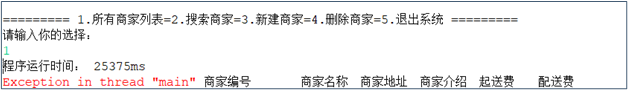
\includegraphics[width=0.8\textwidth]{lianjiechia}
	\caption{优化后}
	\vspace{\baselineskip}
\end{figure}

 
采用连接池后:
\begin{figure}[htbp]
	\centering
	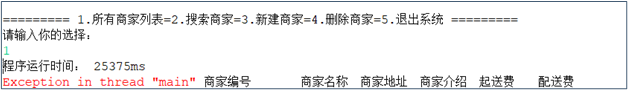
\includegraphics[width=0.8\textwidth]{lianjiechia}
	\caption{优化后}
	\vspace{\baselineskip}
\end{figure}
\section{数据库缓存}
\subsection{背景}

当网站的处理和访问量非常大的时候,数据库的压力就变大了,数据库的连接池,数据库同时处理数据的能力就会受到很大的挑战,一旦数据库承受了其最大承受能力,网站的数据处理效率就会大打折扣。

\subsection{技术原理}
Redis其实就是说把表中经常访问的记录放在了Redis中,然后用户查询时先去查询Redis再去查询MySQL,确实实现了读写分离,也就是Redis只做读操作。由于缓存在内存中,所以查询会很快。

同时还需注意数据库的同步。在对Mysql数据库进行增删改的操作时,会删除redis数据库中相关联的信息,在下次查询时将数据填入redis缓存,做到缓存和数据库的同步。

\subsection{redis优势}
redis缓存在内存中,同时是类似Hashmap的存储方式,查询速度很快。

\subsubsection{使用效果}

压力测试:通过JMeter做压力测试,通过多线程并发不断地给后台发送HTTP请求,测试性能

采用redis前:
\begin{figure}[htbp]
	\centering
	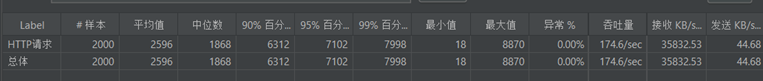
\includegraphics[width=0.8\textwidth]{redisa}
	\caption{优化前}
	\vspace{\baselineskip}
\end{figure}


采用redis后:
\begin{figure}[htbp]
	\centering
	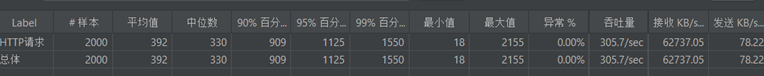
\includegraphics[width=0.8\textwidth]{redisb}
	\caption{优化后}
	\vspace{\baselineskip}
\end{figure}

可以看到吞吐量和延迟都有了很明显的优化效果
\section{积分系统}

\section{修改用户信息}

